\section{Introduction and architecture}
According to Microsoft,  in Windows authentication, credential management
refers to the  underlying process that takes credential material from the user
to  present to the authentication target.  In case of:
\begin{itemize}
    \item a non-domain joined computer:  the authentication target is the
        \emph{Security Accounts Manager} (SAM)~/ref{win:SAM}  database on the local machine. 
    \item  a domain joined computer:  the authentication target is
    the \emph{Domain Controller} through the \emph{WinLogon} service.
\end{itemize}

Security information that is stored locally in the host is located in the
registry~\ref{win:registry} under \verb+HKEY_LOCAL_MACHINE\SECURITY+. Information found in this registry can include:
\begin{itemize}
    \item Policy settings
    \item Default security values
    \item Account information
    \item Cached logon credentials
    \item Copy of the SAM database (write-protected)
\end{itemize}

Windows Server operating systems include a set of security components that make up the Windows security model. These components ensure that applications cannot gain access to resources without authentication and authorization. 

The following diagram shows the components that are required and the paths that credentials take through the system to authenticate the user or process for a successful logon.

\begin{figure}
  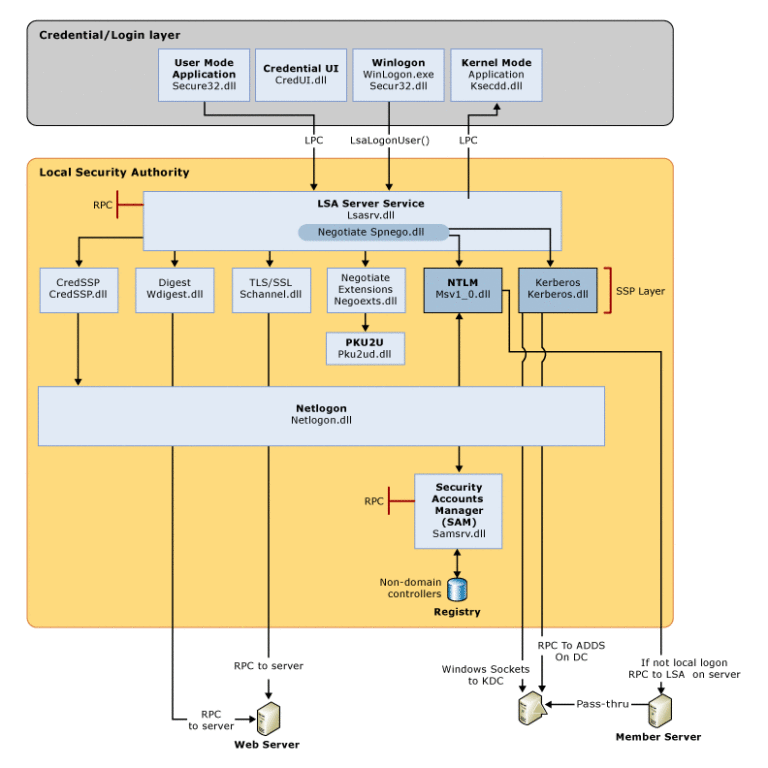
\includegraphics[width=\linewidth]{windows_knowledge/authentication/images/credential.png}
  \caption{Credential process architecture}
  \label{fig:credential-process-architecture}
\end{figure}

\subsection{Credential Provider}
Windows has a list of maybe 2 dozen credential providers to do various tasks, like take your password, handle your smart card, scan your fingerprint, etc. Windows knows what credentials are supported on this machine, so it enumerates them and shows them.

They are all identified by a GUID and stored in \verb+HKEY_LOCAL_MACHINE\SOFTWARE\Microsoft\Windows\CurrentVersion\Authentication\Credential Providers+

\subsection{Local Security Authority}

The LSA is a system component that oversees all the security decisions on your machine. Whenever Windows needs to authenticate a user or verify permissions or what not, the system asks the LSA. It primarily lives in a user mode service: LSASS.

LSASS is kind of dumb. It only has one job, which is to act as a service host. That service that gets hosted is The LSA.

The LSA is *also* a service host, whose job is to host additional services.

So, that LSA service. It's called the LSA server and is backed by lsasrv.dll. If you go look at the files you'll see this is an absolutely massive DLL compared to lsass.exe. That's where all the meat is.

The server has two jobs:
\begin{itemize}
    \item  host an RPC server (shocked face)
    \item manage additional child services. These child services are critical, but less interesting. They are things like netlogon, the key isolation service, or LDAP or KDC on your domain controller. 
\end{itemize} 

Whenever your application makes a security call, like LogonUser, or something like SSPI's \href{https://learn.microsoft.com/en-us/windows/win32/api/sspi/nf-sspi-initializesecuritycontexta}{InitializeSecurityContext}, your process must call this RPC server. Your application doesn't get to touch LSA directly. It goes through some stub calls like LogonUser, which are RPC clients, which communicate to LSA, and then LSA does all the magic.

LSA (server) doesn't strictly know what the magic is. LSA (server) knows how to communicate with clients, but it has to hand the actual work off to plugins called authentication providers.


Can't anyone call RPC? Actually yes. But it turns out the kernel-side RPC server checks the caller's token to make sure it's SYSTEM. 

\subsection{Security Support Provider Interface}

Windows Server operating systems implement a default set of
\emph{authentication security support
providers}~\ref{win:SSP}, which include:
\begin{itemize}
    \item \emph{Negotiate}, 
    \item \emph{Kerberos protocol}
    \item \emph{NTLM}
    \item \emph{Schannel} (secure channel)
    \item \emph{Digest}
\end{itemize}


The protocols used by these providers enable authentication of users,
computers, and services, and the authentication process enables authorized users and services to access resources in a secure manner.

\emph{Applications authenticate users by using the SSPI} to abstract calls for authentication. 
